\documentclass[12pt,a4paper,reqno]{amsart}

% language
\usepackage[greek,english]{babel}
\usepackage[utf8]{inputenc}
\usepackage{alphabeta}

% change default names to greek
\addto\captionsenglish{
    \renewcommand{\contentsname}{Περιεχόμενα}
    \renewcommand{\refname}{Βιβλιογραφία}
    \renewcommand{\datename}{Ημερομηνία:}
    \renewcommand{\urladdrname}{Ιστοσελίδα}
}

% math 
\usepackage{amsmath,amsthm,amssymb,amscd}

% font
\usepackage[cal=euler]{mathalfa}
\usepackage{libertinus-type1}
% \usepackage{txfonts} % for upright greek letters
\usepackage{bm} % for bold symbols
\usepackage{bbm} % for the simply-looking bb symbols

% miscellaneous 
\usepackage{changepage} %for indenting environments
\usepackage{csquotes} % example: \textcquote{}
\usepackage{blkarray}
\setcounter{MaxMatrixCols}{20} % default for pmatrix is 10!!
\usepackage{ytableau}
\usepackage{array} %needed to increase the vertical length in a tabular

% drawing
\usepackage{tikz,tikz-cd}
\usetikzlibrary{shapes.misc, patterns, matrix, calc, intersections,positioning,arrows.meta}
\usepackage{graphics,graphicx}
\usepackage{float} % provides enhanced control and customization options for floating objects such as figures and tables

% colors
\usepackage{xcolor}
\definecolor{darkcandyapplered}{rgb}{0.64, 0.0, 0.0}
\definecolor{midnightblue}{rgb}{0.1, 0.1, 0.44}
\definecolor{mylightblue}{HTML}{336699}
\definecolor{burntorange}{rgb}{0.8, 0.33, 0.0}
\definecolor{iceberg}{rgb}{0.44, 0.65, 0.82}
\definecolor{applegreen}{rgb}{0.55, 0.71, 0.0}
\definecolor{canaryyellow}{rgb}{1.0, 0.94, 0.0}
\definecolor{lightgray}{rgb}{0.83, 0.83, 0.83}

% hrefs
\usepackage{hyperref}
\usepackage[noabbrev,capitalize]{cleveref}
\hypersetup{
    pdftoolbar=true,        
    pdfmenubar=true,        
    pdffitwindow=false,     
    pdfstartview={FitH},  % fits the width of the page to the window
    pdftitle={},
    pdfauthor={},
    pdfsubject={},
    pdfkeywords={},
    pdfnewwindow=true,  % links in new window
    colorlinks=true,  % false: boxed links; true: colored links
    linkcolor=darkcandyapplered,   % color of internal links
    citecolor=midnightblue,  % color of links to bibliography
    urlcolor=cyan,  % color of external links
    linktocpage=true  % changes the links from the section body to the page number
    }

% geometry
\textwidth=16cm 
\textheight=21cm 
\hoffset=-55pt 
\footskip=25pt

% thm envs (you might need to change the path)
\theoremstyle{definition}
\newtheorem{theorem}{Θεώρημα}
\newtheorem{proposition}[theorem]{Πρόταση}
\newtheorem{lemma}[theorem]{Λήμμα}
\newtheorem{corollary}[theorem]{Πόρισμα}
\newtheorem{conjecture}[theorem]{Εικασία}
\newtheorem{problem}[theorem]{Πρόβλημα}
\newtheorem*{claim}{Ισχυρισμός}
\newtheorem{observation}[theorem]{Παρατήρηση}
\newtheorem{definition}[theorem]{Ορισμός}
\newtheorem{question}[theorem]{Ερώτημα}
\newtheorem*{questions}{Ερωτήματα}
\newtheorem*{que}{Ερώτημα}
\newtheorem{example}[theorem]{Παράδειγμα}
\newtheorem{exercise}{Άσκηση}
\newtheorem*{zorn}{Λήμμα του Zorn}
\newtheorem*{example_6.6}{Παράδειγμα~6.6}

\theoremstyle{remark}
\newtheorem*{remark}{Παρατήρηση}

% fixes the correct numbering of environments
\numberwithin{theorem}{section}
\numberwithin{exercise}{section}
\numberwithin{equation}{section}

% math ops 
% fields
\newcommand{\NN}{\mathbbmss{N}} 
\newcommand{\ZZ}{\mathbbmss{Z}} 
\newcommand{\QQ}{\mathbbmss{Q}} 
\newcommand{\RR}{\mathbbmss{R}} 
\newcommand{\CC}{\mathbbmss{C}} 
\newcommand{\KK}{\mathbbmss{K}} 
\newcommand{\FF}{\mathbbmss{F}} 
\newcommand{\HH}{\mathbbmss{H}} 

% symmetric group
\newcommand{\fS}{\mathfrak{S}}  

% calligraphic 
\newcommand{\aA}{\mathcal{A}} 
\newcommand{\bB}{\mathcal{B}}
\newcommand{\cC}{\mathcal{C}}
\newcommand{\dD}{\mathcal{D}}
\newcommand{\eE}{\mathcal{E}}
\newcommand{\fF}{\mathcal{F}}
\newcommand{\hH}{\mathcal{H}}
\newcommand{\iI}{\mathcal{I}}
\newcommand{\lL}{\mathcal{L}}
\newcommand{\oO}{\mathcal{O}}
\newcommand{\pP}{\mathcal{P}}
\newcommand{\qQ}{\mathcal{Q}}
\newcommand{\sS}{\mathcal{S}}
\newcommand{\mM}{\mathcal{M}}
\newcommand{\uU}{\mathcal{U}}

% bold
\newcommand{\bfa}{\mathbf{a}}
\newcommand{\bfe}{\mathbf{e}}
\newcommand{\bfF}{\pmb{F}}
\newcommand{\bfR}{\pmb{R}}
\newcommand{\bfv}{\mathbf{v}}
%\newcommand{\bfx}{\bm{x}}
%\newcommand{\bfx}{\mathbf{x}} 
\newcommand{\bfx}{\pmb{x}}
\newcommand{\bfX}{\pmb{X}}
\newcommand{\bfy}{\pmb{y}}
\newcommand{\bfz}{\pmb{z}}

% roman
\newcommand{\rmA}{\mathrm{A}}
\newcommand{\rmB}{\mathrm{B}}
\newcommand{\rmC}{\mathrm{C}}
\newcommand{\rmD}{\mathrm{D}} 
\newcommand{\rmF}{\mathrm{F}} 
\newcommand{\rmH}{\mathrm{H}} 
\newcommand{\rmh}{\mathrm{h}} 
\newcommand{\rmI}{\mathrm{I}} 
\newcommand{\rmK}{\mathrm{K}}
\newcommand{\rmM}{\mathrm{M}}
\newcommand{\rmP}{\mathrm{P}}  
\newcommand{\rmp}{\mathrm{p}}  
\newcommand{\rmQ}{\mathrm{Q}}  
\newcommand{\rmR}{\mathrm{R}}
\newcommand{\rmS}{\mathrm{S}}
\newcommand{\rmT}{\mathrm{T}}
\newcommand{\rmU}{\mathrm{U}}
\newcommand{\rmV}{\mathrm{V}}
\newcommand{\rmY}{\mathrm{Y}}
\newcommand{\rmZ}{\mathrm{Z}}
\newcommand{\rmz}{\mathrm{z}}

% arrows and symbols 
\renewcommand{\to}{\rightarrow}
\newcommand{\toto}{\longrightarrow}
\newcommand{\mapstoto}{\longmapsto}
\newcommand{\then}{\Rightarrow}
\newcommand{\IFF}{\Leftrightarrow}
\newcommand{\tl}{\tilde}
\newcommand{\wtl}{\widetilde}
\newcommand{\ol}{\overline}
\newcommand{\ul}{\underline}
\newcommand{\oldemptyset}{\emptyset}
\renewcommand{\emptyset}{\varnothing}
\DeclareMathSymbol{\Arg}{\mathbin}{AMSa}{"39} % for arguments 
\newcommand{\onto}{\ensuremath{\twoheadrightarrow}}
\newcommand{\tle}{\trianglelefteq}
\newcommand{\tge}{\trianglerighteq}

% custom ops
\newcommand{\rmKer}{\mathrm{Ker}}
\newcommand{\rmIm}{\mathrm{Im}}
\newcommand{\lcm}{\mathrm{lcm}}
\newcommand{\GL}{\mathrm{GL}}
\newcommand{\ev}{\mathrm{ev}}
\newcommand{\End}{\mathrm{End}}
\newcommand{\rmid}{\mathrm{id}}
\newcommand{\rmspan}{\mathrm{span}}
\newcommand{\Hom}{\mathrm{Hom}}
\newcommand{\Ann}{\mathrm{Ann}}
\newcommand{\Set}{\pmb{\mathrm{Set}}}
\newcommand{\Rmod}{\pmb{\mathrm{mod}}}
\newcommand{\rmrank}{\mathrm{rank}}
\newcommand{\mSpec}{\mathrm{mSpec}}
\newcommand{\Spec}{\mathrm{Spec}}
\newcommand{\tor}{\mathrm{tor}}

% absolute value symbol
\usepackage{mathtools} 
\DeclarePairedDelimiter\abs{\lvert}{\rvert}%
\DeclarePairedDelimiter\norm{\lVert}{\rVert}%
\makeatletter
\let\oldabs\abs
\def\abs{\@ifstar{\oldabs}{\oldabs*}}

% tensor symbol
\newcommand{\tensor}[1]{%
  \mathbin{\mathop{\otimes}\limits_{#1}}%
}

% permutation cycle notation
\ExplSyntaxOn
\NewDocumentCommand{\cycle}{ O{\;} m }
 {
  (
  \alec_cycle:nn { #1 } { #2 }
  )
 }

\seq_new:N \l_alec_cycle_seq
\cs_new_protected:Npn \alec_cycle:nn #1 #2
 {
  \seq_set_split:Nnn \l_alec_cycle_seq { , } { #2 }
  \seq_use:Nn \l_alec_cycle_seq { #1 }
 }
\ExplSyntaxOff

% setminus symbol
\newcommand{\mysetminusD}{\hbox{\tikz{\draw[line width=0.6pt,line cap=round] (3pt,0) -- (0,6pt);}}}
\newcommand{\mysetminusT}{\mysetminusD}
\newcommand{\mysetminusS}{\hbox{\tikz{\draw[line width=0.45pt,line cap=round] (2pt,0) -- (0,4pt);}}}
\newcommand{\mysetminusSS}{\hbox{\tikz{\draw[line width=0.4pt,line cap=round] (1.5pt,0) -- (0,3pt);}}}
\newcommand{\sm}{\mathbin{\mathchoice{\mysetminusD}{\mysetminusT}{\mysetminusS}{\mysetminusSS}}}

% miscellaneous commands
\newcommand{\defn}[1]{{\color{mylightblue}{#1}}}
\newcommand{\toDo}{{\bf\color{red} TODO}}
\newcommand{\toCite}{{\bf\color{green} CITE}}
\newcommand*{\vertbar}{\rule[-1ex]{0.5pt}{2.5ex}} % for matrices with column vectors
\newcommand*{\horzbar}{\rule[.5ex]{2.5ex}{0.5pt}} % for matrices with row vectors
\newcommand{\myblue}[1]{{\color{iceberg}{#1}}}
\newcommand{\myorange}[1]{{\color{burntorange}{#1}}}
\newcommand{\mygreen}[1]{{\color{applegreen}{#1}}}
\newcommand{\myred}[1]{{\color{darkcandyapplered}{#1}}}

% ferrer's diagram
\newcommand{\fdiagram}[1]{
    \begin{tikzpicture}[scale=.7]
        \fill foreach \Z [count=\Y] in {#1}
        {foreach \X in {1,...,\Z} 
        {(\X,-\Y) circle[radius=3pt]}};
    \end{tikzpicture}
}

%
\usepackage{pgfplots}
\pgfplotsset{compat=1.18}

%
\makeatletter
\def\mathcolor#1#{\@mathcolor{#1}}
\def\@mathcolor#1#2#3{%
  \protect\leavevmode
  \begingroup
    \color#1{#2}#3%
  \endgroup
}
\makeatother

% restriction
\newcommand\restr[2]{{% we make the whole thing an ordinary symbol
  \left.\kern-\nulldelimiterspace % automatically resize the bar with \right
  #1 % the function
  \littletaller % pretend it's a little taller at normal size
  \right|_{#2} % this is the delimiter
  }}
\newcommand{\littletaller}{\mathchoice{\vphantom{\big|}}{}{}{}}

% 
\newenvironment{nouppercase}{%
  \let\uppercase\relax%
  \renewcommand{\uppercasenonmath}[1]{}}{}

% titlepage
\title{226: Θεωρία Δακτυλίων και Modules}
\author[Β.~Δ. Μουστακας]{Βασίλης Διονύσης Μουστάκας \\ Πανεπιστήμιο Κρήτης}
\date{23 Απριλίου 2026}
% \urladdr{\href{https://sites.google.com/view/vasmous}{https://sites.google.com/view/vasmous}}

\begin{document}

\begingroup
\def\uppercasenonmath#1{} % this disables uppercase title
\let\MakeUppercase\relax % this disables uppercase authors
\maketitle
\endgroup

\setcounter{section}{7}
\setcounter{theorem}{4}
\setcounter{equation}{5}
\begin{center}
    \textbf{7. Πρότυπα πάνω από περιοχές κύριων ιδεωδών
} (Συνέχεια)
\end{center}

Η απόδειξη της ύπαρξης της διάσπασης σε αναλλοίωτους παράγοντες βασίζεται στο παρακάτω λήμμα, το οποίο αποτελεί μια εκλέπτυνση του Θεωρήματος 7.1.
% \ref{thm:submodules_of_free_modules_are_free_over_PID}.
\begin{lemma}
    \label{lem:aligned_bases}
    Έστω $R$ μια περιοχή κύριων ιδεωδών και $M$ ένα ελεύθερο $R$-πρότυπο τάξης $n$. Αν $N$ είναι υποπρότυπο του $M$, τότε υπάρχει βάση $\{e_1, e_2, \dots, e_n\}$ του $M$, ένας μη αρνητικός ακέραιος $d \le n$ και στοιχεία $a_1, a_2, \dots, a_d \in R$ τέτοια ώστε 
    \begin{itemize}
        \item $a_i \mid a_j$, για κάθε $1 \le i \le j \le d$, και 
        \item το σύνολο $\{a_1e_1, a_2e_2, \dots, a_de_d\}$ αποτελεί βάση του $N$.
    \end{itemize}
\end{lemma}

Η απόδειξη του Λήμματος \ref{lem:aligned_bases}, η οποία παραλείπεται, χρησιμοποιεί τεχνικές γραμμικής άλγεβρας και συγκεκριμένα την \emph{κανονική μορφή Smith} (βλ. \cite[Κεφάλαιο~4]{EKPA_PID}). 
\begin{example}
    \label{ex:aligned_bases}
    Ας δούμε τι ακριβώς μας πληροφορεί το Λήμμα \ref{lem:aligned_bases} στην περίπτωση των αβελιανών ομάδων. Έστω $R = \ZZ$ και $M = \ZZ[i]$. Όπως είδαμε στο Παράδειγμα 5.2 (ε), το $M$ είναι ελεύθερο $\ZZ$-πρότυπο τάξης $2$ με βάση $\{1, i\}$. Στην βάση αυτή, μπορούμε να φανταστούμε το $M$ ως το σύνολο των ζευγών με ακέραιες συντεταγμένες στο (μιγαδικό) επίπεδο
    \[
    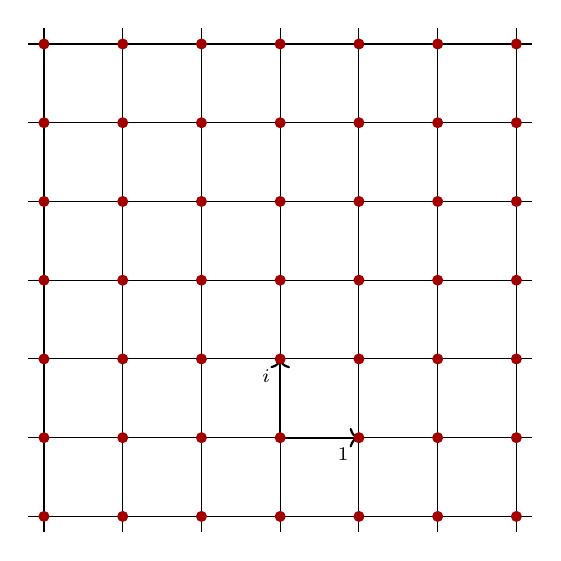
\begin{tikzpicture}[scale=1]
        % Draw grid
        \draw[step=1cm, thin] (-3.2,-3.2) grid (3.2,3.2);

        % Highlight axes
        % \draw[thick] (-2.4,0) -- (2.4,0) node[right] {};
        % \draw[thick] (0,-2.4) -- (0,2.4) node[above] {};
        \draw[->, thick] (0,-2) -- (0,-1) node[below left] {\scriptsize{$i$}};
        \draw[->, thick] (0,-2) -- (1,-2) node[below left] {\scriptsize{$1$}};

        % Plot lattice points (Gaussian integers)
        \foreach \x in {-3,-2,-1,0,1,2,3}
            \foreach \y in {-3,-2,-1,0,1,2,3}
            \fill[darkcandyapplered] (\x,\y) circle (2pt);
    \end{tikzpicture}
    \]
    όπως κάναμε στο Παράδειγμα 2.3. 

    Μια άλλη βάση του $M$ είναι το σύνολο $\{1+2i, i\}$. Πράγματι, κάθε $\alpha + \beta i \in M$ μπορεί να γραφεί ως 
    \[
    \alpha + \beta{i} = \alpha + 2\alpha{i} - 2\alpha{i} + \beta{i} = \alpha\left(
        1 + 2i
    \right) + \underbrace{\left(
        \beta - 2\alpha
    \right)}_{\in \ \ZZ}i
    \]
    και αν 
    \[
    0 = \gamma(1+2i) + \delta{i} = \gamma + (2\gamma+\delta)i
    \]
    τότε $\gamma = \delta = 0$. Στην νέα αυτή βάση, το \textquote{πλέγμα} της προηγούμενης εικόνας παίρνει την μορφή
    \[
    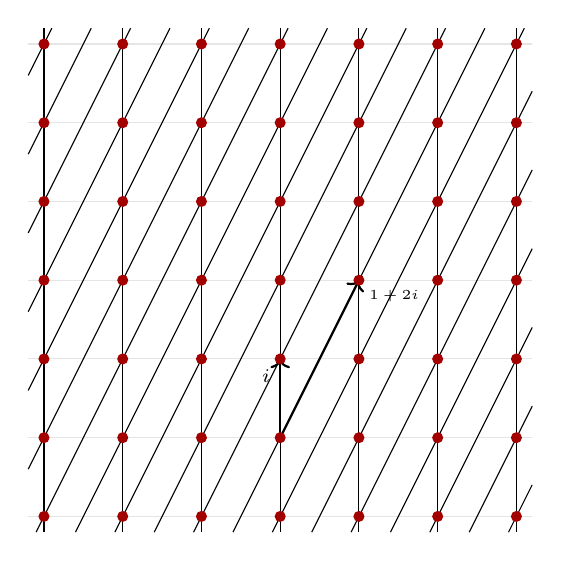
\begin{tikzpicture}[scale=1]

    % Draw grid
        \draw[step=1cm, gray!20, thin] (-3.2,-3.2) grid (3.2,3.2);

    % Draw vertical lines (same as before)
    \foreach \x in {-3,-2,-1,0,1,2,3}
        \draw[thin] (\x,-3.2) -- (\x,3.2);

    % Draw slanted lines parallel to (1,2): y = 2x + c
    \foreach \x in {-3.1,-2.6,-2.1,-1.6,-1.1,-0.6,-0.1}
        \draw[thin] (\x,-3.2) -- (3.2+\x,3.2);
    \foreach \x in {0.4,0.9,1.4,1.9,2.4,2.9}
        \draw[thin] (\x,-3.2) -- (3.2,3.2-2*\x);
    \foreach \y in {-2.4,-1.4,-.4,.6,1.6,2.6}
        \draw[thin] (-3.2,\y) -- (-1.6-\y/2,3.2);
        

    % Basis vectors
    \draw[->, thick] (0,-2) -- (0,-1) node[below left] {\scriptsize{$i$}};
    \draw[->, thick] (0,-2) -- (1,0) node[below right] {\tiny{$1 + 2i$}};

    % Lattice points
    \foreach \x in {-3,-2,-1,0,1,2,3}
            \foreach \y in {-3,-2,-1,0,1,2,3}
            \fill[darkcandyapplered] (\x,\y) circle (2pt);

    \end{tikzpicture}
    \]

    Ας θεωρήσουμε το υποπρότυπο $N = M(1+2i)$. Αυτό είναι ελεύθερο $\ZZ$-πρότυπο με βάση το $\{1+2i, -2+i\}$ (γιατί;), σε συμφωνία με το Θεώρημα 7.1.
    % \ref{thm:submodules_of_free_modules_are_free_over_PID}. 
    Στην βάση αυτή και την αρχική βάση του $M$, τα \textquote{πλέγματα} των δύο αυτών προτύπων μοιάζουν ως εξής
    \[
    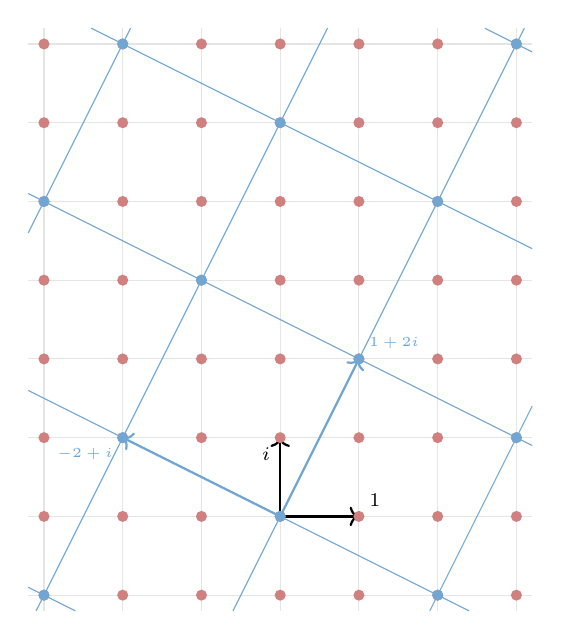
\begin{tikzpicture}[scale=1]
        % Draw grid
        \draw[step=1cm, gray!20, thin] (-3.2,-1.2) grid (3.2,6.2);

        % Highlight axes
        % \draw[thick] (-2.4,0) -- (2.4,0) node[right] {};
        % \draw[thick] (0,-2.4) -- (0,2.4) node[above] {};
        \draw[->, thick] (0,0) -- (0,1) node[below left] {\scriptsize{$i$}};
        \draw[->, thick] (0,0) -- (1,0) node[above right] {\scriptsize{$1$}};

        % Plot lattice points (Gaussian integers)
        \foreach \x in {-3,-2,-1,0,1,2,3}
            \foreach \y in {-1,0,1,2,3,4,5,6}
            \fill[darkcandyapplered!50] (\x,\y) circle (2pt);

        \draw[->, iceberg, thick] (0,0) -- (1,2) node[above right] {\tiny{$1+2i$}};
        \draw[->, iceberg, thick] (0,0) -- (-2,1) node[below left] {\tiny{$-2+i$}};

        \draw[iceberg, thin] (-.6,-1.2) -- (3.1,6.2);
        \draw[iceberg, thin] (-3.1,-1.2) -- (.6,6.2);
        \draw[iceberg, thin] (-3.2,3.6) -- (-1.9,6.2);
        \draw[iceberg, thin] (3.2,1.4) -- (1.9,-1.2);

        \draw[iceberg, thin] (-3.2,1.6) -- (2.4,-1.2);
        \draw[iceberg, thin] (-3.2,-.9) -- (-2.6,-1.2);
        \draw[iceberg, thin] (-3.2,4.1) -- (3.2,.9);
        \draw[iceberg, thin] (-2.4,6.2) -- (3.2,3.4);
        \draw[iceberg, thin] (2.6,6.2) -- (3.2,5.9);

        \fill[iceberg] (1,2) circle (2pt);
        \fill[iceberg] (2,4) circle (2pt);
        \fill[iceberg] (3,6) circle (2pt);
        \fill[iceberg] (0,0) circle (2pt);
        \fill[iceberg] (3,1) circle (2pt);
        \fill[iceberg] (2,-1) circle (2pt);
        \fill[iceberg] (-2,1) circle (2pt);
        \fill[iceberg] (-1,3) circle (2pt);
        \fill[iceberg] (0,5) circle (2pt);
        \fill[iceberg] (-3,-1) circle (2pt);
        \fill[iceberg] (-3,4) circle (2pt);
        \fill[iceberg] (-2,6) circle (2pt);
    \end{tikzpicture}
    \]

    Οι βάσεις $\{1, i\}$ και $\{1+2i, -2+i\}$ των $M$ και $N$, αντίστοιχα, δεν ικανοποιούν τις συνθήκες του Λήμματος \ref{lem:aligned_bases}. Μια ακόμη βάση του $N$ είναι το σύνολο $\{1+2i,5i\}$ (γιατί;). Η βάση αυτή μαζί με την βάση $\{1+2i, i\}$ του $M$ που είδαμε παραπάνω ικανοποιούν τις συνθήκες του Λήμματος \ref{lem:aligned_bases} με $a_1 = 1$ και $a_2 = 5$, με την εικόνα που προκύπτει να είναι η εξής 
    \[
    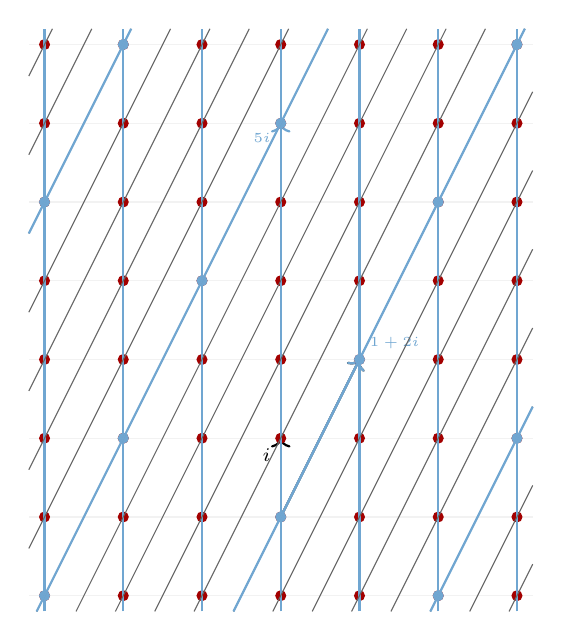
\begin{tikzpicture}[scale=1]
        % Draw grid
        \draw[step=1cm, gray!10, thin] (-3.2,-1.2) grid (3.2,6.2);

        % basis for M
        \draw[->, thick] (0,0) -- (1,2) node[below left] {};
        \draw[->, thick] (0,0) -- (0,1) node[below left] {\scriptsize{$i$}};

        % basis for N
        \draw[->, iceberg, thick] (0,0) -- (1,2) node[above right] {\tiny{$1+2i$}};
        \draw[->, iceberg, thick] (0,0) -- (0,5) node[below left] {\tiny{$5i$}};

        % Plot lattice points (Gaussian integers)
        \foreach \x in {-3,-2,-1,0,1,2,3}
            \foreach \y in {-1,0,1,2,3,4,5,6}
            \fill[darkcandyapplered] (\x,\y) circle (2pt);

        %sublattice
        \fill[iceberg] (1,2) circle (2pt);
        \fill[iceberg] (2,4) circle (2pt);
        \fill[iceberg] (3,6) circle (2pt);
        \fill[iceberg] (0,0) circle (2pt);
        \fill[iceberg] (3,1) circle (2pt);
        \fill[iceberg] (2,-1) circle (2pt);
        \fill[iceberg] (-2,1) circle (2pt);
        \fill[iceberg] (-1,3) circle (2pt);
        \fill[iceberg] (0,5) circle (2pt);
        \fill[iceberg] (-3,-1) circle (2pt);
        \fill[iceberg] (-3,4) circle (2pt);
        \fill[iceberg] (-2,6) circle (2pt);

        \foreach \x in {-3,-2,-1,0,1,2,3}
            \draw[iceberg,thick] (\x,-1.2)--(\x,6.2);
        \foreach \x in {0,1,2,3,4,5}
            \draw[black!60] (-3.1+.5*\x,-1.2)--(0.6+.5*\x,6.2);
        \foreach \x in {0,1,2,3,4,5,6}
            \draw[black!60] (-.1+.5*\x,-1.2)--(3.2,5.4-1*\x);
        \foreach \x in {0,1,2,3,4,5,6}
            \draw[black!60] (-3.2,-.4+1*\x)--(.1-.5*\x,6.2);
        
        \foreach \x in {0,5}
            \draw[iceberg,thick] (-3.1+.5*\x,-1.2)--(0.6+.5*\x,6.2);
        \foreach \x in {4}
            \draw[iceberg,thick] (-.1+.5*\x,-1.2)--(3.2,5.4-1*\x);
        \foreach \x in {4}
            \draw[iceberg,thick] (-3.2,-.4+1*\x)--(.1-.5*\x,6.2);
    \end{tikzpicture}
    \]
    Το Λήμμα \ref{lem:aligned_bases} μας πληοροφορεί ότι μπορούμε \emph{πάντα} να βρούμε δύο τέτοιες βάσεις.
\end{example}

\begin{proof}[Απόδειξη του Θεωρήματος 7.3 (Ύπαρξη αναλλοίωτων παραγόντων)]
    Θα αποδείξουμε την ύπα\-ρξη της διάσπασης σε αναλλοίωτους παράγοντες. Για το λόγο αυτό, υποθέτουμε ότι το $M$ έχει ένα σύνολο με $d$ γεννήτορες. Από την Πρόταση 5.4 έπεται ότι υπάρχει ένα ελεύθερο $R$-πρότυπο $F$ τάξης $d$ και ένας $R$-επιμορφισμός $\phi : F \to M$ και από το πρώτο θεώρημα ισομορφισμού, έπεται ότι $M \cong F/N$, όπου $N = \ker(\phi)$.

    Εφαρμόζοντας το Λήμμα \ref{lem:aligned_bases} στο $F$ και το $N$, μπορούμε να γράψουμε 
    \begin{align*}
    F &= Re_1 \oplus Re_2 \oplus \cdots \oplus Re_d \\
    N &= Ra_1e_1 \oplus Ra_2e_2 \oplus \cdots \oplus Ra_\ell{e_\ell},
    \end{align*}
    για κάποια $e_1, e_2, \dots, e_d \in M$, $\ell \le d$ και $a_1, a_2, \dots, a_\ell \in R$ τέτοια ώστε $a_i \mid a_{i+1}$, για κάθε $1 \le i \le \ell-1$. Από την Άσκηση 21, έχουμε
    \begin{align*}
        M &\cong F/N \\
        &= \frac{Re_1 \oplus Re_2 \oplus \cdots \oplus Re_\ell \oplus Re_{\ell+1} \oplus \cdots \oplus Re_d}{Ra_1e_1 \oplus Ra_2e_2 \oplus \cdots \oplus Ra_\ell{e_\ell}\oplus 0 \oplus \cdots \oplus 0} \\
        &\cong \frac{Re_1}{Ra_1e_1} \oplus \frac{Re_2}{Ra_2e_2} \oplus \cdots \oplus \frac{Re_\ell}{Ra_\ell e_\ell} \oplus Re_{\ell+1} \oplus \cdots \oplus Re_{d} \\
        &\cong R^{d-\ell} \oplus R/(a_1) \oplus R/(a_2) \oplus \cdots \oplus R/(a_\ell)
    \end{align*}
    και το ζητούμενο έπεται.
\end{proof}

Στο σημείο αυτό, μπορούμε να αποδείξουμε την μοναδικότητα της τάξης του $M$ ως $R$-πρότυπο.
\begin{proof}[Απόδειξη Θεωρήματος 7.3 (Μοναδικότητα τάξης)]
    Έχοντας κατά νου την διάσπαση (7.4), αν
    \[
    M \cong R^n \oplus M_\tor \cong R^k \oplus M_\tor,  
    \]
    για κάποια $n, k \ge 0$, τότε 
    \[
    M/M_\tor \cong R^n \cong R^k.
    \]
    Από το Θεώρημα 5.6 (μοναδικότητα τάξης ελεύθερου προτύπου), έπεται ότι $n=k$.
\end{proof}

Η απόδειξη της μοναδικότητας της διάσπασης σε αναλλοίωτους παράγοντες βασίζεται στο παρακάτω λήμμα. 
\begin{lemma}
    \label{lem:uniqueness_of_invariant_factors}
    Έστω $R$ μια περιοχή κύριων ιδεωδών και $p \in R$ ένα ανάγωγο στοιχείο. Αν $M$ είναι κυκλικό $R$-πρότυπο με $\Ann_R(M) = (a)$, για κάποιο $a \in R$, τότε 
    \[
    \dim_{R/(p)}\left(
        M/pM
    \right) = \begin{cases}
        1, &\ \text{αν $p \mid a$} \\
        0, &\ \text{διαφορετικά},
    \end{cases}
    \]
    όπου $pM \coloneqq (p)M$.
\end{lemma}

\begin{proof}[Απόδειξη]
    Στην απόδειξη του Θεωρήματος 5.6 είδαμε ότι το $M/pM$ είναι $R/(p)$-πρότυπο. Επειδή το $p$ είναι ανάγωγο, το Λήμμα 2.14 μας πληροφορεί ότι το ιδεώδες $(p)$ του $R$ είναι μεγιστικό και κατά συνέπεια το $R/(p)$ είναι σώμα από την Πρόταση 1.10. Επομένως, έχει νόημα να υπολογίσουμε την ποσότητα $\dim_{R/(p)}\left(
        M/pM
    \right)$.

    Παρατηρούμε ότι 
    \[
    pM \cong \frac{(p) + (a)}{(a)}
    \]
    (γιατί;). Επομένως, από το τρίτο θεώρημα ισομορφισμού, έπεται ότι 
    \[
    \frac{M}{pM} \cong \frac{R/(a)}{\left((p) + (a)\right)/(a)} \cong \frac{R}{(p) + (a)}.
    \]
    Αν $p \mid a$, τότε $(p) + (a) = (p)$ και γι αυτό 
    \[
    \dim_{R/(p)}\left(
        M/pM
    \right) = \dim_{R/(p)}\left(
        R/(p)
    \right) = 1.
    \]

    Διαφορετικά, υποθέτουμε ότι $p \nmid a$. Στην περίπτωση αυτή, ισχυριζόμαστε ότι $(p) + (a) = R$ και κατά συνέπεια 
    \[
    \dim_{R/(p)}\left(
        M/pM
    \right) = \dim_{R/(p)}\left(
        R/R
    \right) = \dim_{R/(p)}(0) = 0.
    \]
    Πράγματι, επειδή ο $R$ είναι περιοχή κύριων ιδεωδών, έχουμε \[
    (p) + (a) = (d),
    \]
    για κάποιο $d \in R$. Επομένως, $(p) \subseteq (d)$ που σημαίνει ότι $d \mid p$. Όμως, το $p$ είναι ανάγωγο και γι αυτό οι μόνοι διαιρέτες του είναι τα αντιστρέψιμα στοιχεία και τα συντροφικά του. Αν τα $d$ και $a$ είναι συντροφικά, τότε $d = up$ για κάποιο $u \in R^\times$. Όμως, 
    \[
    (a) \subseteq (d) = (up) = (p),
    \] 
    που σημαίνει ότι $p \mid a$, το οποίο είναι αδύνατο. Άρα, $d \in R^\times$ και γι αυτό $(d) = R$.
\end{proof}

\begin{proof}[Απόδειξη του Θεωρήματος 7.3 (Μοναδικότητα αναλλοίωτων παραγόντων)]
    Χωρίς βλάβη της γε\-νικότητας, μπορούμε να υποθέσουμε ότι\footnote{Στην περίπτωση αυτή το $M$ ονομάζεται \defn{πρότυπο στρέψης} (βλ. Άσκηση 18).} $M = M_\tor$ και θεωρούμε δύο διασπάσεις σε αναλλοίωτους παράγοντες 
    \[
    M \cong M_1 \oplus M_2 \oplus \cdots \oplus M_\ell \cong N_1 \oplus N_2 \oplus \cdots \oplus N_k,
    \]
    όπου $\Ann_R(M_i) = (a_i), \Ann_R(N_j) = (b_j)$ για κάθε $1 \le i \le \ell$ και $1 \le j \le k$ με $a_i \mid a_{i+1}$ και $b_j \mid b_{j+1}$ για κάθε $1 \le i \le \ell-1$ και $1 \le j \le k-1$, αντίστοιχα.

    Αρχικά, θα δείξουμε ότι $\ell = k$. Επειδή ο $R$ είναι περιοχή κύριων ιδεωδών, από το Θεώρημα 2.12, έπεται ότι είναι και περιοχή μοναδικής παραγοντοποίησης. Συνεπώς, υπάρχει ανάγωγο $p \in R$ τέτοιο ώστε $p \mid a_1$ και κατά συνέπεια $p \mid a_i$, για κάθε $1 \le i \le \ell$. Από το Λήμμα \ref{lem:uniqueness_of_invariant_factors} έπεται ότι 
    \[
    \dim_{R/(p)}\left(
            M_i/pM_i
        \right) = 1
    \]
    για κάθε $1 \le i \le \ell$. Άρα, 
    \begin{align*} 
        \dim_{R/(p)}\left(
            M/pM
        \right) &= 
        \dim_{R/(p)}\left(
            \frac{M_1 \oplus M_2 \oplus \cdots \oplus M_\ell}{pM_1 \oplus pM_2 \oplus \cdots \oplus pM_\ell} 
        \right)\\
        &= 
        \dim_{R/(p)}\left(
            \frac{M_1}{pM_1} \oplus \frac{M_2}{pM_2} \oplus \cdots \oplus \frac{M_\ell}{pM_\ell}
        \right) \\ 
        &= \dim_{R/(p)}\left(
            \frac{M_1}{pM_1}
            \right) + \dim_{R/(p)}\left(
            \frac{M_2}{pM_2}
            \right) + \cdots + \dim_{R/(p)}\left(
            \frac{M_\ell}{pM_\ell}
            \right) \\
        &= \ell,
    \end{align*}
    όπου η δεύτερη ισότητα έπεται από την Άσκηση 21. Όμως, από το Λήμμα \ref{lem:uniqueness_of_invariant_factors} έπεται επίσης ότι 
    $\dim_{R/(p)}\left(
            N_j/pN_j
        \right) \leq 1$, για κάθε $1 \le j \le k$. Συνεπώς, 
    \[
    \ell = \dim_{R/(p)}\left(
            M/pM
        \right) = \sum_{j=1}^k \dim_{R/(p)}\left(
            N_j/pN_j
        \right) \le k.
    \]
    Ομοίως, $k \le \ell$ και η ισότητα έπεται.

    Στη συνέχεια, θα δείξουμε ότι $(a_i) = (b_i)$ για κάθε $1 \le i \le \ell$. Σταθεροποιούμε ένα υποδείκτη $1 \le i \le \ell$ και παρατηρούμε ότι 
    \[
    a_iM_1 = a_iM_2 = \cdots = a_iM_i = 0
    \]
    Πράγματι, εξ υποθέσεως 
    \[
    (a_i) \subseteq (a_{i-1}) \subseteq \cdots \subseteq (a_1).
    \]
    Όμως, για κάθε $1 \le j \le i$, $a_jM_j = 0$, διότι το $a_j$ είναι γεννήτορας του $\Ann_R(M_j)$ και το ζητούμενο έπεται. Επομένως, 
    \[
    a_iM \cong a_iM_{i+1} \oplus \cdots \oplus a_iM_\ell
    \]
    και εξ' υποθέσεως
    \begin{equation}  
        \label{eq:structure_help}
        a_iM \cong a_iN_1 \oplus a_iN_2 \oplus \cdots \oplus a_iN_\ell.
    \end{equation}
    Επειδή τα $a_iM_j$ και $a_iN_j$ είναι κυκλικά πρότυπα, απαριθμώντας γεννήτορες και στα δύο μέλη της Ταυτότητας \eqref{eq:structure_help}, έπεται ότι τουλάχιστον $i$ προσθεταίοι του δεξιού μέλους είναι μηδενικά πρότυπα. 
    
    Ισχυριζόμαστε ότι $a_iN_i = 0$. Πράγματι, αν $a_iN_i \neq 0$, τότε $a_i \notin \Ann_R(N_i) = (b_i)$. Όμως, εξ υποθέσεως  
    \[
    (b_\ell) \subseteq (b_{\ell-1}) \subseteq \cdots \subseteq (b_{i+1}) \subseteq (b_i)
    \]
    και γι αυτό $a_i \notin (b_j) = \Ann_R(N_j)$ για κάθε $j \ge i$. Επομένως, $a_iN_j \neq 0$, για κάθε $j \ge i$. Με άλλα λόγια, βρήκαμε τουλάχιστον $\ell -i +1$ μη μηδενικούς προσθεταίους. Ισοδύναμα, αυτό σημαίνει ότι υπάρχουν το πολύ $i-1$ μηδενικοί προσθεταίοι, το οποίο είναι αδύνατο. 
    
    Επειδή $a_iN_i = 0$ έπεται ότι $(a_i) \subseteq (b_i)$. Ομοίως, $(b_i) \subseteq (a_i)$. Άρα $(a_i) = (b_i)$ και το ζητούμενο έπεται.
\end{proof}

Μένει να αποδείξουμε την ύπαρξη και την μοναδικότητα της διάσπασης σε στοιχειώδεις διαιρέτες. Τώρα που γνωρίζουμε την διάσπαση σε αναλλοίωτους παράγοντες, το πρώτο είναι ουσιαστικά εφαρμογή του κινεζικού θεωρήματος υπολοίπων.
\begin{proof}[Απόδειξη του Θεωρήματος 7.3 (Ύπαρξη στοιχειωδών διαιρετών)]
    Υποθέτουμε ότι 
    \[
    M \cong R^n \oplus R/(a_1) \oplus R/(a_2) \oplus \cdots \oplus R/(a_\ell),
    \]
για κάποια $n, \ell \ge 0$ και κάποια μη μηδενικά, μη αντιστρέψιμα $a_1, a_2, \dots, a_\ell \in R$ τέτοια ώστε $a_i \mid a_{i+1}$, για κάθε $1 \le i \le \ell-1$. Επειδή ο $R$ είναι περιοχή κύριων ιδεωδών, από το Θεώρημα 2.12 έπεται ότι είναι και περιοχή μονοσήμαντης παραγοντοποίησης και γι αυτό 
\[
a_i = \prod_{\substack{p \in R \\ \text{το p είναι πρώτο στοιχείο του $R$}}} p^{\lambda_i^{(p)}}.
\]
Το (πεπερασμένο) πλήθος των διαφορετικών πρώτων στοιχείων που εμφανίζονται είναι τουλά\-χιστον $i$, διότι $a_1 \mid a_2 \mid \cdots \mid a_\ell$. Από το κινέζικο θεώρημα υπολοίπων, έπεται ότι 
\begin{equation}
    \label{eq:elementary_divisors_help}
    R/(a_i) \cong \bigoplus_{\substack{p \in R \\ \text{το p είναι πρώτο στοιχείο του $R$}}} R/(p^{\lambda_i^{(p)}})
\end{equation}
για κάθε $1 \le i \le \ell$. Η διάσπαση (7.2) έπεται ομαδοποιώντας τους προσθεταίους στην διάσπαση (7.1) ως προς πρώτα στοιχεία, χρησιμοποιώντας την Ταυτότητα \eqref{eq:elementary_divisors_help}.
\end{proof}

Η διαδικασία αυτή μπορεί να \textquote{αντιστραφεί} για να κατασκευάσει κανείς τους αναλλοίωτους παράγοντες δοθέντων των στοιχειωδών διαιρετών, όπως έγινε στο Παράδειγμα 7.4. Έτσι έπεται η μοναδικότητα της διάσπασης σε στοιχειώδεις διαιρέτες. Οι λεπτομέρειες αφήνονται ως άσκηση.

\begin{remark}
    Η ακολουθία θετικών ακεραίων $\lambda = (\lambda_1,\lambda_2, \dots, \lambda_k)$ που εμφανίζεται στη διάσπαση σε στοιχειώδεις διαιρέτες και ικανοποιεί τη συνθήκη 
    \[
    \lambda_1 \ge \lambda_2 \ge \cdots \ge \lambda_k
    \]
    ονομάζεται \defn{διαμέριση ακεραίου} (integer partition). Αν $\lambda_1 + \lambda_2 + \cdots + \lambda_k = n$, τότε λέμε ότι το $\lambda$ είναι διαμέριση του $n$. Για παράδειγμα, οι διαμερίσεις του 4 είναι 
    \[
    (1,1,1,1), \ (2,1,1), \ (2,2), \ (3,1), \ (4).
    \]
    Οι διαμερίσεις ακεραίων παίζουν κεντρικό ρόλο στη θεωρία αριθμών, την αλγεβρική συνδυαστική και τη θεωρία αναπαραστάσεων των συμμετρικών ομάδων (βλ., για παράδειγμα, \cite[Ενότητα~6]{StaAC}).
\end{remark}

Το Θεώρημα 7.3 έχει δύο πολύ σημαντικές εφαρμογές. Στην περίπτωση όπου $R=\ZZ$, ταξινομεί όλες τις πεπερασμένα παραγόμενες αβελιανές ομάδες. 
\begin{example}
\label{ex:abelian_groups}
Ας ταξινομήσουμε όλες τις αβελιανές ομάδες τάξης $1800 = 2^33^25^2$ χρησιμοποιώντας τους στοιχειώδεις διαιρέτες. Έχουμε 
\[
\renewcommand{\arraystretch}{1.2}
\begin{array}{c|c|c}
    p^n & \text{διαμερίσεις του $n$} & \text{αβελιανές ομάδες τάξης $p^n$} \\ \hline
    2^3 & (1,1,1)                    & \ZZ_2\oplus\ZZ_2\oplus\ZZ_2 \\ 
        & (2,1)                      & \ZZ_4 \oplus \ZZ_2 \\
        & (3)                        & \ZZ_8 \\\hline
    3^2 & (1,1)                      & \ZZ_3 \oplus \ZZ_3 \\
        & (2)                        & \ZZ_9 \\ \hline 
    5^2 & (1,1)                      & \ZZ_5 \oplus \ZZ_5 \\ 
        & (2)                        & \ZZ_{25}
\end{array} \ .
\]
Παίρνοντας όλους τους πιθανούς συνδυασμούς των αβελιανών ομάδων από τη δεξιά στήλη προκύπτουν όλες οι αβελιανές ομάδες τάξης $1800$
\[
\renewcommand{\arraystretch}{1.2}
\begin{array}{c|c|c|c}
    \text{αβελιανή ομάδα} & \lambda^{(2)} & \lambda^{(3)} & \lambda^{(5)} \\ \hline
    \ZZ_2 \oplus \ZZ_2 \oplus \ZZ_2 \oplus \ZZ_3 \oplus \ZZ_3 \oplus \ZZ_5 \oplus \ZZ_5 & (1,1,1) & (1,1) & (1,1) \\ \hline
    \ZZ_2 \oplus \ZZ_2 \oplus \ZZ_2 \oplus \ZZ_3 \oplus \ZZ_3 \oplus \ZZ_{25} & (1,1,1) & (1,1) & (2) \\ \hline
    \ZZ_2 \oplus \ZZ_2 \oplus \ZZ_2 \oplus \ZZ_9 \oplus \ZZ_5 \oplus \ZZ_5 & (1,1,1) & (2) & (1,1) \\ \hline
    \ZZ_2 \oplus \ZZ_2 \oplus \ZZ_2 \oplus \ZZ_9 \oplus \ZZ_{25} & (1,1,1) & (2) & (2) \\ \hline
    \ZZ_4 \oplus \ZZ_2 \oplus \ZZ_3 \oplus \ZZ_3 \oplus \ZZ_5 \oplus \ZZ_5 & (2,1) & (1,1) & (1,1) \\ \hline
    \ZZ_4 \oplus \ZZ_2 \oplus \ZZ_3 \oplus \ZZ_3 \oplus \ZZ_{25} & (2,1) & (1,1) & (2) \\ \hline
    \ZZ_4 \oplus \ZZ_2 \oplus \ZZ_9 \oplus \ZZ_5 \oplus \ZZ_5 & (2,1) & (2) & (1,1) \\ \hline
    \ZZ_4 \oplus \ZZ_2 \oplus \ZZ_9 \oplus \ZZ_{25} & (2,1) & (2) & (2) \\ \hline
    \ZZ_8 \oplus \ZZ_3 \oplus \ZZ_3 \oplus \ZZ_5 \oplus \ZZ_5 & (3) & (1,1) & (1,1) \\ \hline
    \ZZ_8 \oplus \ZZ_3 \oplus \ZZ_3 \oplus \ZZ_{25} & (3) & (1,1) & (2) \\ \hline
    \ZZ_8 \oplus \ZZ_9 \oplus \ZZ_5 \oplus \ZZ_5 & (3) & (2) & (1,1) \\ \hline
    \ZZ_8 \oplus \ZZ_9 \oplus \ZZ_{25} & (3) & (2) & (2)
\end{array} \ .
\]
\end{example}

Στην περίπτωση όπου $R = F[x]$, όπου $F$ είναι ένα σώμα, το Θεώρημα 7.3 ταξινομεί όλα τα πεπερασμένα παραγόμενα $F[x]$-πρότυπα, δηλαδή διανυσματικούς χώρους πάνω από το $F$ εφοδιασμένους με κάποιο $T \in \End_F(V)$. Στην περίπτωση αυτή, η διάσπαση σε
\begin{itemize}
    \item αναλλοίωτους παράγοντες ονομάζεται \emph{ρητή κανονική μορφή} (rational canonical form)
    \item στοιχειώδεις διαιρέτες ονομάζεται \emph{κανονική μορφή Jordan} (Jordan canonical form).
\end{itemize} 
Οι δύο αυτές διασπάσεις είναι πολύ σημαντικές στην γραμμική άλγεβρα. Στις σημειώσεις αυτές δε θα τις μελετήσουμε και γι αυτό παραπέμπουμε στα \cite[Ενότητα 3, Μέρος II]{EKPA_LA}, \cite[Κεφάλαιο 7]{EKPA_PID} και \cite[Κεφάλαιο 12]{DF04}.


\begin{thebibliography}{99}
    \bibitem{EKPA_LA}
    Δ. Α. Βάρσος, Δ. Ι. Δεριζιώτης, Ι. Π. Εμμανουήλ, Μ. Π. Μαλιάκας, Α. Δ. Μελάς και Ο. Π. Ταλέλλη, 
    \emph{Μια Εισαγωγή στην Γραμμική Άλγεβρα}, 
    Εκδόσεις Σοφία, 2012.
    %
    \bibitem{DF04}
    D. S. Dummit και R. M. Foote, 
    \textit{Abstract algebra},
    third edition, Wiley, 2004. 
    %
    \bibitem{EKPA_PID}
    Μ. Π. Μαλιάκας, και Ο. Π. Ταλέλλη, 
    \emph{Πρότυπα πάνω από Περιοχές Κυρίων Ιδεωδών και Εφαρμογές}, 
    Εκδόσεις Σοφία, 2009.
    %
    \bibitem{StaAC}
    R. P. Stanley,
    \emph{Algebraic Combinatorics; Walks, Trees, Tableaux and More},
    second edition, Undergraduate Texts in Mathematics, Springer, 2018.
\end{thebibliography}
\end{document}